% Figure -- molecule encoder contrast (CheMeleon vs MACE). \input{} from Ch4 sec:profiling-mol.
% Generated by figures/scripts/fig_ch4_mol_encoders.py (CheMeleon RankMe re-run env, 2026-06-04).
\begin{figure}[tbp]
\centering
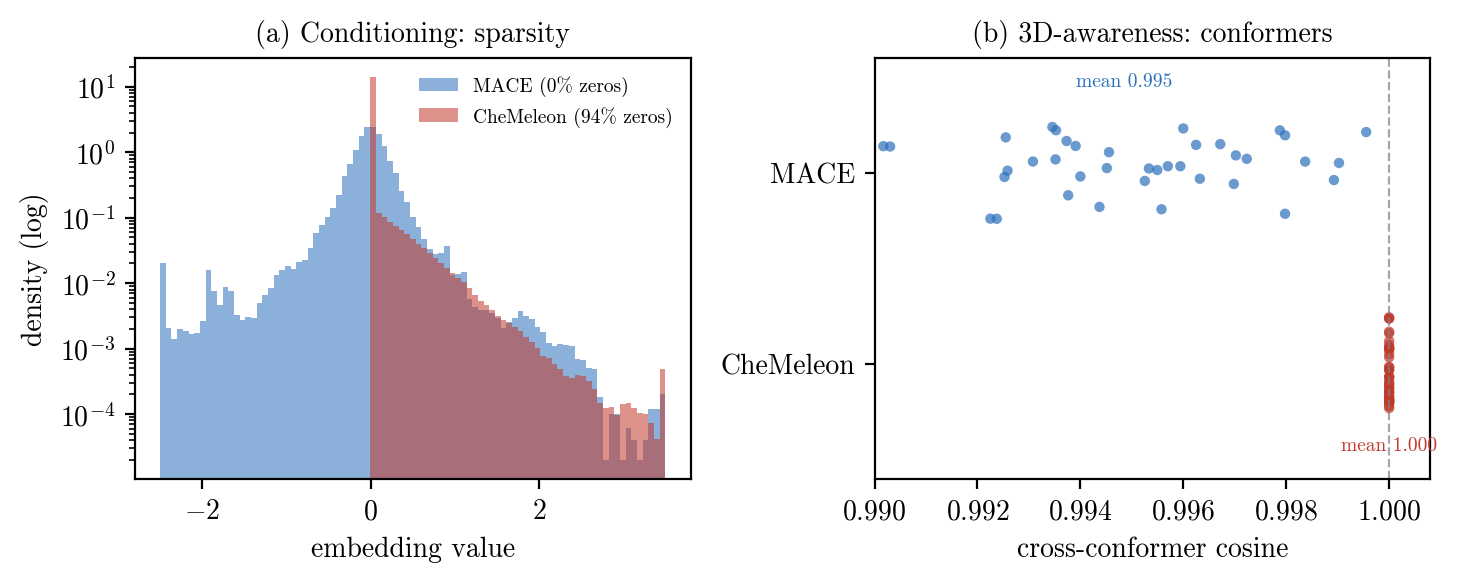
\includegraphics[width=\textwidth]{figures/fig_ch4_mol_encoders.png}
\caption{\textbf{The two molecule encoders fail in opposite ways.} (a)~Conditioning (Q3): CheMeleon's output is almost entirely zeros, so the cosine alignment runs over a sparse, shifting subset of dimensions, while MACE is dense. (b)~3D-awareness (Q1): each point is one molecule's mean cosine between its 3D conformers. CheMeleon is conformer-invariant by construction (cosine~$1.000$), so REPA against it cannot teach geometry; MACE moves only slightly (mean cosine~$0.995$), confirming a real but weak 3D signal. Neither is a clean alignment target.}
\label{fig:profiling-mol}
\end{figure}
